\documentclass[dvipsnames, hidelinks]{beamer}

% Enables the use of colour.
\usepackage{xcolor}
% Syntax high-lighting for code. Requires Python's pygments.
\usepackage{minted}
% Enables the use of umlauts and other accents.
\usepackage[utf8]{inputenc}
% Diagrams.
\usepackage{tikz}
% Settings for captions, such as sideways captions.
\usepackage{caption}
% Symbols for units, like degrees and ohms.
\usepackage{gensymb}
% Latin modern fonts - better looking than the defaults.
\usepackage{lmodern}
% Allows for columns spanning multiple rows in tables.
\usepackage{multirow}
% Better looking tables, including nicer borders.
\usepackage{booktabs}
% More math symbols.
\usepackage{amssymb}
% More math layouts, equation arrays, etc.
\usepackage{amsmath}
% More math fonts, like mathbb.
\usepackage{amsfonts}
% More theorem environments.
\usepackage{amsthm}
% More column formats for tables.
\usepackage{array}
% Adjust the sizes of box environments.
\usepackage{adjustbox}
% Better looking single quotes in verbatim and minted environments.
\usepackage{upquote}
% Better blank space decisions.
\usepackage{xspace}
% Better looking tikz trees.
\usepackage{forest}
% URLs.
\usepackage{hyperref}
% For plotting.
\usepackage{pgfplots}

% Various tikz libraries.
% For drawing mind maps.
\usetikzlibrary{mindmap}
% For adding shadows.
\usetikzlibrary{shadows}
% Extra arrows tips.
\usetikzlibrary{arrows.meta}
% Old arrows.
\usetikzlibrary{arrows}
% Automata.
\usetikzlibrary{automata}
% For more positioning options.
\usetikzlibrary{positioning}
% Creating chains of nodes on a line.
\usetikzlibrary{chains}
% Fitting node to contain set of coordinates.
\usetikzlibrary{fit}
% Extra shapes for drawing.
\usetikzlibrary{shapes}
% For markings on paths.
\usetikzlibrary{decorations.markings}
% For advanced calculations.
\usetikzlibrary{calc}

% GMIT colours.
\definecolor{gmitblue}{RGB}{20,134,225}
\definecolor{gmitred}{RGB}{220,20,60}
\definecolor{gmitgrey}{RGB}{67,67,67}

% Change some style options.
\usetheme{metropolis}
\usemintedstyle{manni}
\setbeamercolor{structure}{fg=gmitblue}
\setbeamercolor{frametitle}{fg=white, bg=gmitred}
\setbeamercolor{alerted text}{fg=gmitblue}
\usefonttheme[onlymath]{serif}

% \citeurl can be used to a clickable short url to a slide as a reference.
\renewcommand\footnoterule{}
\newcommand{\citeurl}[1]{\let\thefootnote\relax\footnotetext{\tiny \textcolor{gmitgrey}{\href{http://#1}{#1}}}}
\newcommand{\citeeg}[1]{\let\thefootnote\relax\footnotetext{\tiny \textcolor{gmitgrey}{#1}}}

% A basic horizontal rule.
\newcommand{\hr}{\rule{\textwidth}{0.5pt}}

% Prevent minted from showing errors.
\makeatletter
\expandafter\def\csname PYGdefault@tok@err\endcsname{\def\PYGdefault@bc##1{{\strut ##1}}}
\makeatother

\begin{document}
  \title{Examples of Deterministic Finite Automata}
  \subtitle{}
  \author{ian.mcloughlin@gmit.ie}
  \date{}

  \begin{frame}
    \titlepage
  \end{frame}

  %!TEX root = slides.tex

\title{Graph Theory}
\subtitle{}
\author{ian.mcloughlin@gmit.ie}
\date{}


\begin{frame}
	\titlepage
\end{frame}

\begin{frame}
	\frametitle{Topics}
	\tableofcontents
\end{frame}

\section{Graphs}

\begin{frame}{Seven Bridges of K{\"o}nigsberg}
	\begin{center}
		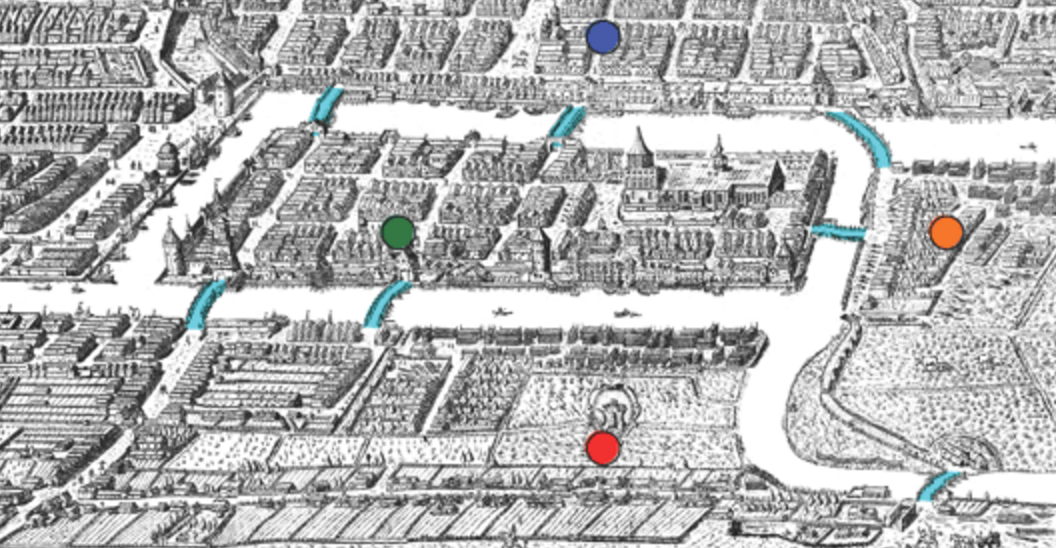
\includegraphics[width=9cm]{img/konigsberg.png}
	\end{center}
	Is it possible to walk through the city crossing each of the seven bridges once and only once?
		\citeurl{www.nature.com/nbt/journal/v29/n11}
\end{frame}

\begin{frame}{Leonhard Euler}
  \begin{columns}
    \begin{column}{0.25\textwidth}
      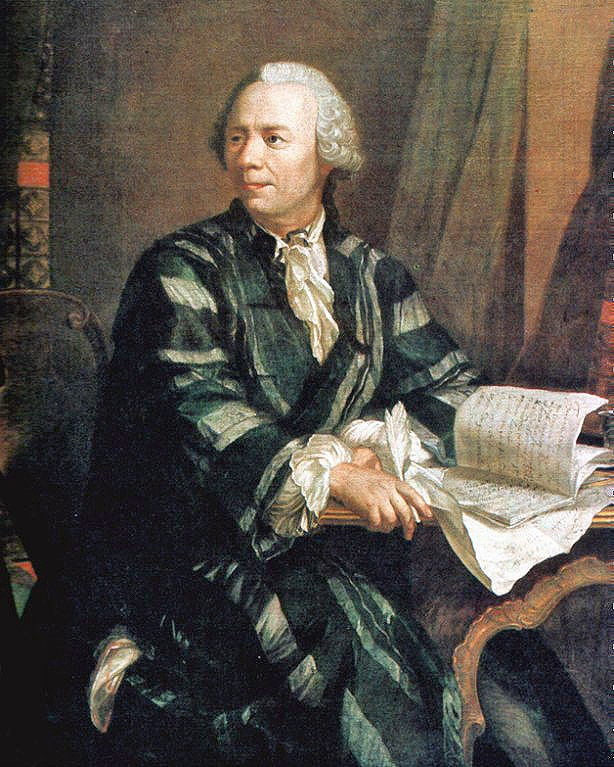
\includegraphics[height=1.8in]{img/euler.jpg}
    \end{column}
    \begin{column}{0.6\textwidth}
      \begin{itemize}
    	 \item Born 1707 in Basel, Switzerland.
        \vspace{0.25cm}
    	 \item Euler's identity: $\mathrm{e}^{i \pi} + 1 = 0$.
        \vspace{0.25cm}
    	 \item Solved the Bridges of K{\"o}nigsberg problem.
        \vspace{0.25cm}
        \item It's not possible to cross all bridges once and once only.
      \end{itemize}
    \end{column}
  \end{columns}
  \citeurl{https://en.wikipedia.org/wiki/Leonhard\_Euler}
\end{frame}

\begin{frame}{Graph of K{\"o}nigsberg}
  \begin{adjustbox}{max width={0.9\textwidth},center} 
    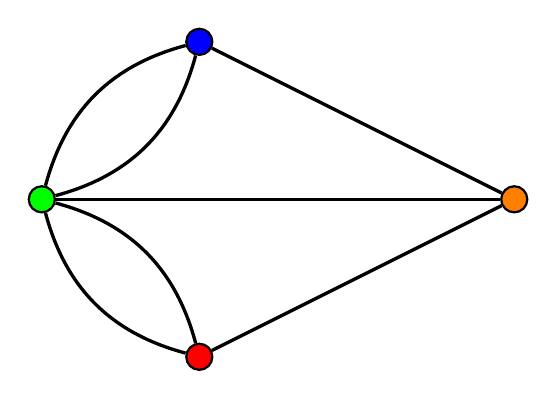
\begin{tikzpicture}
			\begin{scope}[every node/.style={circle,thick,draw}]
		    \node[fill=green] (A) at (0,0) {};
		    \node[fill=blue] (B) at (2,2) {};
		    \node[fill=orange] (C) at (6,0) {};
		    \node[fill=red] (D) at (2,-2) {};
			\end{scope}
			\begin{scope}[every edge/.style={draw=black,very thick}]
		    \path (A) edge[bend right=30] (B);
    		\path (A) edge[bend left=30] (B);
		    \path (A) edge[bend right=30] (D);
		    \path (A) edge[bend left=30]  (D);
		    \path (B) edge (C);
		    \path (A) edge (C);
		    \path (D) edge (C);
	    \end{scope}
    \end{tikzpicture}
  \end{adjustbox}
\end{frame}


\begin{frame}{Graph definition}
	\begin{definition}
	A \emph{graph} consists of a finite set $V$ and a set $E$ of 2-subsets of $V$.
	\end{definition}
	\vspace{0.25cm}
	\begin{description}
		\item[Vertices] -- the elements of the set $V$ are called vertices.
		\vspace{0.25cm}
		\item[Edges] -- the elements of $E$ are called edges.
		\vspace{0.25cm}
		\item[$G = (V,E)$] -- this is the way we write the graph $G$ consists of the vertex set $V$ and the edge set $E$.
	\end{description}
\end{frame}

\begin{frame}{Sets of K{\"o}nigsberg}
$$ V = \{Green, Blue, Orange, Red\} $$
\begin{align*}
E = \{&\\
			&\{Green, Blue\}, \{Green, Blue\}, \{Green, Red\},\\
      &\{Green, Red\}, \{Blue, Orange\}, \{Green, Orange\},\\
      &\{Red, Orange\}\\
      \}&
\end{align*}
\end{frame}

\begin{frame}{Adjanceny list}
	\begin{center}
	\begin{tabular}{l|l|l|l}
	Green & Blue & Orange & Red \\
	\hline
	Blue & Green & Blue & Green \\
	Orange & Orange & Green & Orange \\
	Red & & Red & 
	\end{tabular}
	\end{center}
\end{frame}

\begin{frame}{Defining different types of graphs}
	
	\begin{block}{Our definition of a graph}
	The definition given above for a graph is not consistent with looped edges, directed edges or repeated edges. We only need to make small changes to the definition of a graph to allow for directed edges and repeated edges.
	\end{block}
	
	\begin{description}
		\item[Repeated edges] are edges that start and end at the same vertices.
		\item[Directed edges] are edges where a direction is added.
		\item[Looped edges] begin and end at the same vertex.
	\end{description}
	
	The application will determine the definition we want to use.
\end{frame}


\begin{frame}{A better example}
  \begin{adjustbox}{max width={0.9\textwidth},center} 
    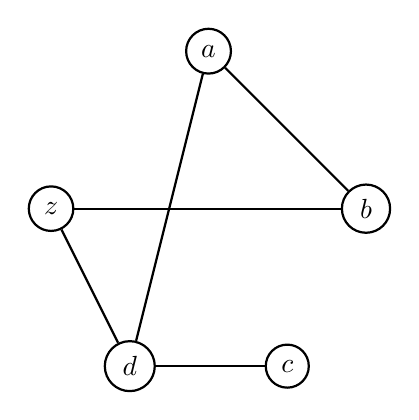
\begin{tikzpicture}
      \begin{scope}[every node/.style={circle,thick,draw}]
        \node (a) at (2,4) {$a$};
        \node (b) at (4,2) {$b$};
        \node (c) at (3,0) {$c$};
        \node (d) at (1,0) {$d$};
        \node (z) at (0,2) {$z$};
      \end{scope}
      \begin{scope}[every edge/.style={draw=black,thick}]
        \path (a) edge (b);
        \path (a) edge (d);
        \path (b) edge (z);
        \path (c) edge (d);
        \path (d) edge (z);
      \end{scope}
    \end{tikzpicture}
  \end{adjustbox}
  \vspace{0.1cm}
  \begin{block}{Exercise}
	Determine the vertex set, edge set and adacency list of this graph.
  \end{block}
  
  \citeurl{global.oup.com/booksites/content/9780198507185/}
\end{frame}


\begin{frame}{Degree of a vertex}

	\begin{definition}
		The degree of a vertex is the number of edges that contain it.
	\end{definition}
	  
  \begin{center}
    \begin{columns}
      \begin{column}{0.2\textwidth}
        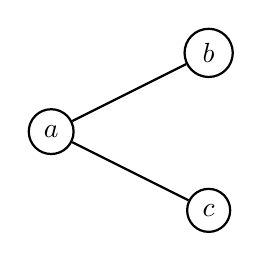
\begin{tikzpicture}
          \begin{scope}[every node/.style={circle,thick,draw}]
            \node (a) at (0,0) {$a$};
            \node (b) at (2,1) {$b$};
            \node (c) at (2,-1) {$c$};
          \end{scope}
          \begin{scope}[every edge/.style={draw=black,thick}]
            \path (a) edge (b);
            \path (a) edge (c);
          \end{scope}
        \end{tikzpicture}
      \end{column}
      \begin{column}{0.5\textwidth}
          The degree of the vertex $a$ is 2.
      \end{column}
    \end{columns}
  \end{center}

  \begin{block}{Exercise}
    For each of the vertices on the previous slide, determine its degree.
  \end{block}

\end{frame}


\begin{frame}{Functions}

	\begin{definition}
		Suppose that $X$ and $Y$ are sets.
		We say we have a function $f$ from $X$ to $Y$ if for each $x$ in $X$ we can specify a unique element in $Y$, which we denote by $f(x)$.
	\end{definition}

	\begin{center}
		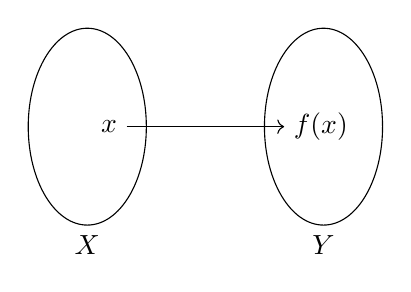
\begin{tikzpicture}
			\draw (0,0) ellipse (0.75 and 1.25);
			\draw (0,-1.5) node {$X$};
			\draw (3,0) ellipse (0.75 and 1.25);
			\draw (3,-1.5) node {$Y$};

			\draw [->]  (0.5,0) node[anchor=east] {$x$} -- (2.5,0) node[anchor=west] {$f(x)$};
		\end{tikzpicture}
	\end{center}

\end{frame}



\begin{frame}{Bijections}

	\begin{definition}
		A bijection is function $f$ from a set $X$ to a set $Y$ where both of the following are true:
			\begin{itemize}
				\item every $y$ in $Y$ is a value $f(x)$ for at most one $x$ in $X$.
				\item every $y$ in $Y$ is a value $f(x)$ for at least one $x$ in  $X$.
			\end{itemize}
	\end{definition}

	\begin{center}
		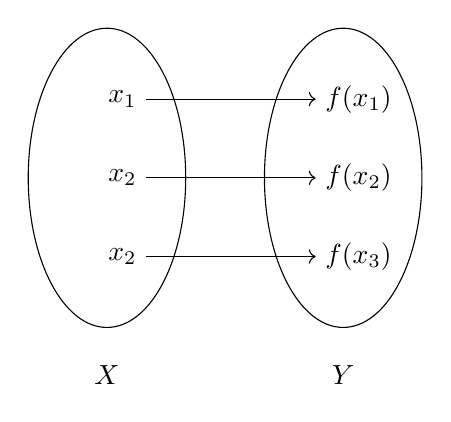
\begin{tikzpicture}
			\draw (0,0) ellipse (1 and 1.9);
			\draw (0,-2.5) node {$X$};
			\draw (3,0) ellipse (1 and 1.9);
			\draw (3,-2.5) node {$Y$};

			\draw [->]  (0.5,1) node[anchor=east] {$x_1$} -- (2.65,1) node[anchor=west] {$f(x_1)$};
			\draw [->]  (0.5,0) node[anchor=east] {$x_2$} -- (2.65,0) node[anchor=west] {$f(x_2)$};
			\draw [->]  (0.5,-1) node[anchor=east] {$x_2$} -- (2.65,-1) node[anchor=west] {$f(x_3)$};
		\end{tikzpicture}
	\end{center}

\end{frame}


\begin{frame}{Isomorphism}

	\begin{definition}
		Two graphs $G_1$ and $G_2$ are said to be isomorphic when there is a bijection $\alpha$ for the vertex set $V_1$ of $G_1$ to the vertex set $V_2$ of $G_2$ such that $\{\alpha (x) , \alpha (y) \}$ is an edge of $G_2$ if and only if $(x,y)$ is an edge of $G_1$.
	\end{definition}
	  
  \begin{center}
    \begin{columns}
      \begin{column}{0.3\textwidth}
        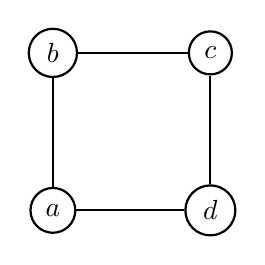
\begin{tikzpicture}
          \begin{scope}[every node/.style={circle,thick,draw}]
            \node (a) at (0,0) {$a$};
            \node (b) at (0,2) {$b$};
            \node (c) at (2,2) {$c$};
            \node (d) at (2,0) {$d$};
          \end{scope}
          \begin{scope}[every edge/.style={draw=black,thick}]
            \path (a) edge (b);
            \path (b) edge (c);
            \path (c) edge (d);
            \path (d) edge (a);
          \end{scope}
        \end{tikzpicture}
      \end{column}
      
      \begin{column}{0.3\textwidth}
        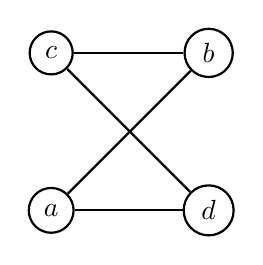
\begin{tikzpicture}
          \begin{scope}[every node/.style={circle,thick,draw}]
            \node (a) at (0,0) {$a$};
            \node (c) at (0,2) {$c$};
            \node (b) at (2,2) {$b$};
            \node (d) at (2,0) {$d$};
          \end{scope}
          \begin{scope}[every edge/.style={draw=black,thick}]
            \path (b) edge (c);
            \path (c) edge (d);
            \path (b) edge (a);
            \path (d) edge (a);
          \end{scope}
        \end{tikzpicture}
      \end{column}
      
      \begin{column}{0.3\textwidth}
        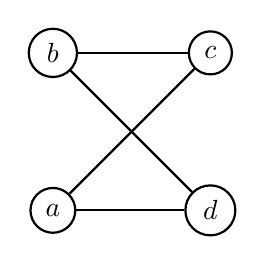
\begin{tikzpicture}
          \begin{scope}[every node/.style={circle,thick,draw}]
            \node (a) at (0,0) {$a$};
            \node (b) at (0,2) {$b$};
            \node (c) at (2,2) {$c$};
            \node (d) at (2,0) {$d$};
          \end{scope}
          \begin{scope}[every edge/.style={draw=black,thick}]
            \path (b) edge (c);
            \path (b) edge (d);
            \path (c) edge (a);
            \path (d) edge (a);
          \end{scope}
        \end{tikzpicture}
      \end{column}
    \end{columns}
  \end{center}

\end{frame}


\begin{frame}{Sum of degrees}

	\begin{theorem}
		The sum of the degrees of the vertices of a graph $G = (V,E)$ is equal to twice the number of edges:
			\[ \sum_{\mathrm{v} \in V} \delta (\mathrm{v}) = 2 | E | \]
	\end{theorem}

	\begin{columns}
		\begin{column}{0.75\textwidth}
			\begin{proof}
				The degree $\delta (\mathrm{v})$ of a vertex $\mathrm{v}$ is equal to the number of edges incident on it.
				Every edge is incident on two vertices.
				So every edge contributes $1$ to the degrees of two distinct vertices.
				Therefore every edge contributes $2$ to the sum total of the degrees of all the vertices.
			\end{proof}
		\end{column}
		\begin{column}{0.2\textwidth}
			\begin{center}
        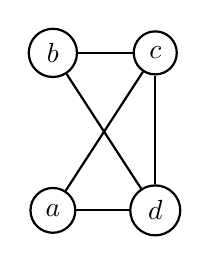
\begin{tikzpicture}
          \begin{scope}[every node/.style={circle,thick,draw}]
            \node (a) at (0,0) {$a$};
            \node (b) at (0,2) {$b$};
            \node (c) at (1.3,2) {$c$};
            \node (d) at (1.3,0) {$d$};
          \end{scope}
          \begin{scope}[every edge/.style={draw=black,thick}]
            \path (b) edge (c);
            \path (b) edge (d);
            \path (d) edge (c);
            \path (c) edge (a);
            \path (d) edge (a);
          \end{scope}
        \end{tikzpicture}
			\end{center}
		\end{column}
	\end{columns}
\end{frame}

\begin{frame}{Handshaking lemma}
	\begin{definition}
		A vertex is an odd vertex if its degree is odd, and it is an even vertex if its degree is even.
		The set of all odd vertices is denoted $V_o$ and the set of all even vertices is denoted $V_e$.
	\end{definition}
	\begin{center}
		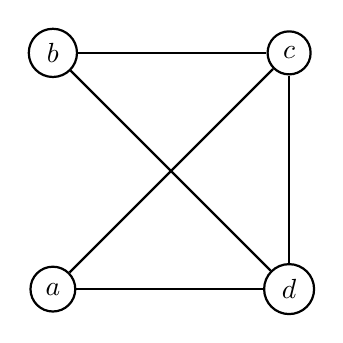
\begin{tikzpicture}
			\begin{scope}[every node/.style={circle,thick,draw}]
				\node (a) at (0,0) {$a$};
				\node (b) at (0,3) {$b$};
				\node (c) at (3,3) {$c$};
				\node (d) at (3,0) {$d$};
			\end{scope}
			\begin{scope}[every edge/.style={draw=black,thick}]
				\path (b) edge (c);
				\path (b) edge (d);
				\path (d) edge (c);
				\path (c) edge (a);
				\path (d) edge (a);
			\end{scope}
		\end{tikzpicture}
	\end{center}
	\begin{block}{Exercise}
		Which of the above vertices are even, and which are odd?
	\end{block}
\end{frame}

\begin{frame}{Handshaking lemma}

	\begin{lemma}
		The number of odd vertices $| V_o |$ in a graph is even.
	\end{lemma}

	\begin{proof}
		The sets $V_o$ and $V_e$ are disjoint (i.e.\ they don't have any elements in common.)
		Also, every vertex is either in $V_o$ or $V_e$.
		Therefore $V = V_o \cup V_e$ and $|V| = |V_o| + |V_e|$.
		
		Furthermore:
			\[ \sum_{\mathrm{v} \in V_o} \delta(\mathrm{v}) + \sum_{\mathrm{v} \in V_e} \delta(\mathrm{v}) = 2 |E| \]

		Both $2|E|$ and $\sum_{\mathrm{v} \in V_e} \delta(\mathrm{v})$ are even, so $\sum_{\mathrm{v} \in V_o} \delta(\mathrm{v})$ must be.
		Since $\delta(\mathrm{v})$ is odd for every $\mathrm{v}$ in $V_o$, this must mean that $|V_o|$ is even.
	\end{proof}

\end{frame}


\begin{frame}{Isomorphism: degrees}

	\begin{block}{Exercise}
		Determine if these two graphs are isomorphic.

		\begin{columns}
			\begin{column}{0.5\textwidth}
				\begin{center}
	        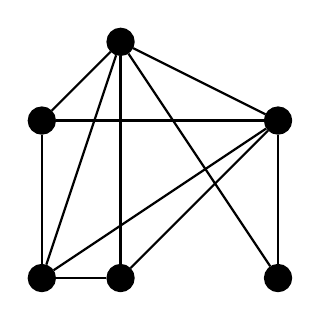
\begin{tikzpicture}
	          \begin{scope}[every node/.style={circle,thick,draw,fill}]
	            \node (a) at (0,1) {};
	            \node (b) at (0,4) {};
	            \node (c) at (2,1) {};
	            \node (d) at (2,3) {};
	            \node (e) at (-1,1) {};
	            \node (f) at (-1,3) {};
	          \end{scope}
	          \begin{scope}[every edge/.style={draw=black,thick}]
	            \path (a) edge (b);
	            \path (a) edge (d);
	            \path (a) edge (e);
	            \path (b) edge (c);
	            \path (b) edge (d);
 	            \path (b) edge (e);
 	            \path (b) edge (f);
 	            \path (c) edge (d);
 	            \path (d) edge (e);           
 	            \path (d) edge (f);
 	            \path (e) edge (f);
	          \end{scope}
	        \end{tikzpicture}
				\end{center}
			\end{column}
			\begin{column}{0.5\textwidth}
				\begin{center}
	        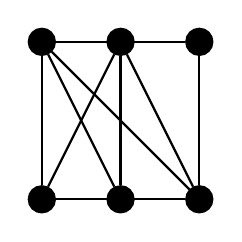
\begin{tikzpicture}
	          \begin{scope}[every node/.style={circle,thick,draw,fill}]
	            \node (a) at (0,0) {};
	            \node (b) at (0,2) {};
	            \node (c) at (1,0) {};
	            \node (d) at (1,2) {};
	            \node (e) at (2,0) {};
	            \node (f) at (2,2) {};
	          \end{scope}
	          \begin{scope}[every edge/.style={draw=black,thick}]
	            \path (a) edge (b);
	            \path (a) edge (e);
	            \path (a) edge (d);
	            \path (b) edge (c);
	            \path (b) edge (d);
 	            \path (b) edge (e);
 	            \path (b) edge (f);
 	            \path (c) edge (d);
 	            \path (d) edge (e);
 	            \path (b) edge (f); 	            
 	            \path (e) edge (f);
	          \end{scope}
	        \end{tikzpicture}
				\end{center}
			\end{column}
		\end{columns}
	\end{block}
\end{frame}

\section{Paths and Cycles}

\begin{frame}{Walks}
  
  \begin{definition}
    A \emph{walk} in a graph is a sequence of vertices
      \[ v_1, v_2, \ldots, v_k \]
    such that $v_i$ and $v_{i+1}$ are adjacent for $1 \leq i < k$.
  \end{definition}
  
  For instance, in the following graph $a,b,c,d,b,f$ is a walk.
  \begin{center}
    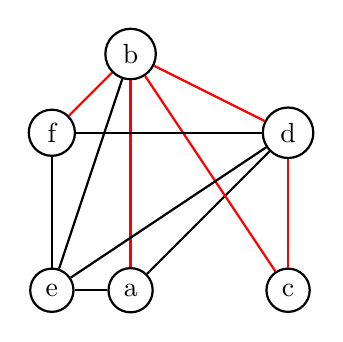
\begin{tikzpicture}
    \begin{scope}[every node/.style={circle,thick,draw}]
      \node (a) at (0,1) {a};
      \node (b) at (0,4) {b};
      \node (c) at (2,1) {c};
      \node (d) at (2,3) {d};
      \node (e) at (-1,1) {e};
      \node (f) at (-1,3) {f};
    \end{scope}
    \begin{scope}[every edge/.style={draw=black,thick}]
      \path (a) edge[red] (b);
      \path (a) edge (d);
      \path (a) edge (e);
      \path (b) edge[red] (c);
      \path (b) edge[red] (d);
      \path (b) edge (e);
      \path (b) edge[red] (f);
      \path (c) edge[red] (d);
      \path (d) edge (e);           
      \path (d) edge (f);
      \path (e) edge (f);
    \end{scope}
    \end{tikzpicture}
  \end{center}

\end{frame}

\begin{frame}{Paths}
  
  \begin{definition}
    A \emph{path} is a walk where each vertex is distinct.
  \end{definition}
  
  For instance, in the following graph $a,b,c,d$ is a path.
  \begin{center}
    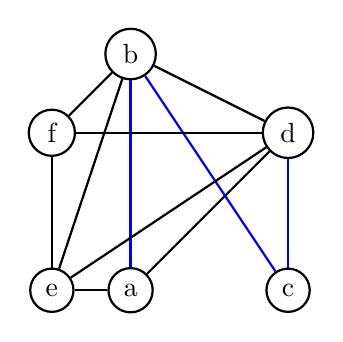
\begin{tikzpicture}
    \begin{scope}[every node/.style={circle,thick,draw}]
    \node (a) at (0,1) {a};
    \node (b) at (0,4) {b};
    \node (c) at (2,1) {c};
    \node (d) at (2,3) {d};
    \node (e) at (-1,1) {e};
    \node (f) at (-1,3) {f};
    \end{scope}
    \begin{scope}[every edge/.style={draw=black,thick}]
    \path (a) edge[blue] (b);
    \path (a) edge (d);
    \path (a) edge (e);
    \path (b) edge[blue] (c);
    \path (b) edge (d);
    \path (b) edge (e);
    \path (b) edge (f);
    \path (c) edge[blue] (d);
    \path (d) edge (e);           
    \path (d) edge (f);
    \path (e) edge (f);
    \end{scope}
    \end{tikzpicture}
  \end{center}
\end{frame}


\begin{frame}{Cycles}
  
  \begin{definition}
    A \emph{cycle} is a walk where each vertex is distinct, except for the start and end vertices being equal.
  \end{definition}
  
  For instance, in the following graph $a,b,c,d,a$ is a path.
  \begin{center}
    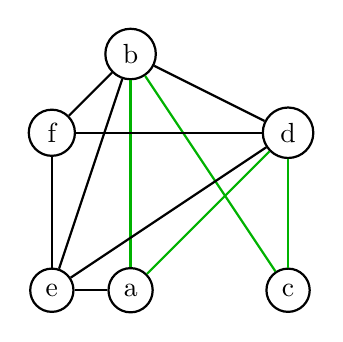
\begin{tikzpicture}
    \begin{scope}[every node/.style={circle,thick,draw}]
    \node (a) at (0,1) {a};
    \node (b) at (0,4) {b};
    \node (c) at (2,1) {c};
    \node (d) at (2,3) {d};
    \node (e) at (-1,1) {e};
    \node (f) at (-1,3) {f};
    \end{scope}
    \begin{scope}[every edge/.style={draw=black,thick}]
    \path (a) edge[green!70!black] (b);
    \path (a) edge[green!70!black] (d);
    \path (a) edge (e);
    \path (b) edge[green!70!black] (c);
    \path (b) edge (d);
    \path (b) edge (e);
    \path (b) edge (f);
    \path (c) edge[green!70!black] (d);
    \path (d) edge (e);           
    \path (d) edge (f);
    \path (e) edge (f);
    \end{scope}
    \end{tikzpicture}
  \end{center}
\end{frame}


\begin{frame}{Hamiltonian cycles}
  
  \begin{definition}
    A \emph{Hamiltonian cycle} is a cycle that contains all of vertices of the graph.
  \end{definition}
  
  For instance, in the following graph $a,b,c,d,f,e,a$ is a path.
  \begin{center}
    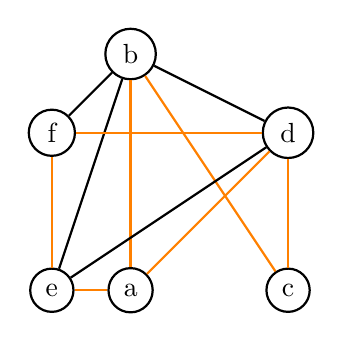
\begin{tikzpicture}
    \begin{scope}[every node/.style={circle,thick,draw}]
    \node (a) at (0,1) {a};
    \node (b) at (0,4) {b};
    \node (c) at (2,1) {c};
    \node (d) at (2,3) {d};
    \node (e) at (-1,1) {e};
    \node (f) at (-1,3) {f};
    \end{scope}
    \begin{scope}[every edge/.style={draw=black,thick}]
    \path (a) edge[orange] (b);
    \path (a) edge[orange] (d);
    \path (a) edge[orange] (e);
    \path (b) edge[orange] (c);
    \path (b) edge (d);
    \path (b) edge (e);
    \path (b) edge (f);
    \path (c) edge[orange] (d);
    \path (d) edge (e);           
    \path (d) edge[orange] (f);
    \path (e) edge[orange] (f);
    \end{scope}
    \end{tikzpicture}
  \end{center}
\end{frame}


\section{Trees}

\section{Colouring}

\section{Sorting}

\section{Searching}

\section{Shortest Paths}
 
\end{document}
 